% !TeX root = ../../main.tex
\documentclass[class=article, crop=false]{standalone}
\begin{document}
\subsection{Interval Complex}

Starting from a Coxeter group $W$ generated by $S$, we wish to give $W$ a labelled--poset structure and use the constructions from the previous section. The edge labelled Hasse diagram for $W$ will embed in to the Cayley graph $\Cay(W,S)$, and it is useful to be able to swap between these two objects, as we will do. First we must define an order on our group $W$.
\begin{definition}[Word length in a group]
    For a group $G$ generated by $S$, the word length with respect to $S$ is the function $l_S:G\to \mathbb{Z}$ where $l_S(g) = \min\{k \mid s_1s_2\ldots s_k=g \,,\, s_i \in S \}$.
\end{definition}

We will often omit the $S$ in $l_S$ where it is obvious from context.

\begin{definition}[Order on a group]
    For a group $G$ generated by $S$, we define the order $x \leq y \iff l(x) + l(x^{-1}y) = l(y)$.
\end{definition}

It can be readily checked that this does indeed define an order on $G$. This order encodes closeness to $e \in G$ along geodesics in $\Cay(G,S)$. We have $x \leq y$ precisely when there exists a geodesic in $\Cay(G, S)$ from $e$ to $y$ with $x$ as an intermediate vertex, or to put it another way, when a minimal factorisation of $x$ in to elements of $S$ is a prefix of a minimal factorisation of $y$.
For some $w \in W$ we define the poset $[1,w]^W$ to be the interval in $W$ up to $w$ with respect to this order. We give this poset an edge labelling such that the edge between $w$ and $ws$ is labelled $s$ for any $s \in S$. The Hasse diagram thus embeds in to $\Cay(W,S)$.

We apply the steps from \cref{sec:poset_cx} to $[1,w]^W$ to form a space.

\begin{definition}[Interval Complex]
    For a Coxeter group $W$, and $w \in W$, we call $K_{W_w} \coloneq K([1,w]^W)$ the \emph{interval complex} where $K([1,w]^W)$ is as in \cref{def:poset_complex}.
    \label{def:interval_complex}
\end{definition}

Note that in \cite{paolini_salvetti_kpi1_2021}  $K_{W_w}$ is denoted $K_W$. We will later show that this notation is justified, in that there is no dependence, up to homotopy equivalence, of $K_{W_w}$ on $w$. For now, we will stick with the notation as we have defined it.
Certain properties of the poset permit a simplified notation for the simplices within $K_{W_w}$. In this context, for two chains $C=(C_1 \leq C_2 \leq \cdots \leq C_m)$ and $C^\prime = (C_1^\prime \leq C_2^\prime \leq \cdots \leq C_n^\prime)$ we have $\mathcal{L}(C) = \mathcal{L}(C^\prime)$ exactly when $(C_1)^{-1}C_m = (C_1^\prime)^{-1}C_n^\prime$. Thus, we can label 1--simplices in $K_{W_w}$ with group elements $x \in [1,w]^W$, we can label 2--simplices with factorisations of group elements in $[1,w]^W$ in to two parts (with the first part also in $[1,w]^W$) and so on. We denote an n--simplex $[x_1 | x_2 | \cdots | x_n]$ as in \cite[Definition 2.8]{paolini_salvetti_kpi1_2021}. This notation also gives the gluing of the faces of $[x_1 | x_2 | \cdots | x_n]$ in the following way. A codimention 1 face of $[x_1 | x_2 | \cdots | x_n]$ is a subchain of $x_1 \leq x_1x_2 \leq \cdots \leq x_1x_2\ldots x_n$ consisting of $n-1$ elements. There are three ways to obtain such a subchain.
\begin{enumerate}
    \item \label{item:gluing_step_1} Remove the first element of the chain to get $x_2 \leq x_2x_3 \leq \cdots \leq x_2x_3\ldots x_n$
    \item \label{item:gluing_step_2} Remove the last element of the chain to get $x_1 \leq x_1x_2 \leq \cdots \leq x_1x_2\ldots x_{n-1}$.
    \item \label{item:gluing_step_3} Multiply two adjacent elements $x_i$ and $x_{i+1}$ to get the chain $x_1 \leq \cdots \leq x_1 \ldots x_{i-1} \leq x_1 \ldots x_{i-1}x_ix_{i+1} \leq \cdots \leq x_1\cdots x_n$ 
\end{enumerate}

So the $n$--simplex $[x_1 | x_2 | \cdots | x_n]$ glues to $[x_2|x_3|\cdots|x_n]$, $[x_1|x_2|\cdots|x_{n-1}]$ and $[x_1| \cdots | x_ix_{i+1} | \cdots |x_n]$ for all $i<n$.

The particular poset group intervals $[1,w]^W$ we will consider will be \emph{balanced}. A balanced group interval is such that  $x \in [1,w]^W$ iff $l(g^{-1}x) + l(x) = l(g)$. I.e.~all minimal factorisation of $x \in [1,w]^W$ also appear as a suffix in a minimal factorisation of $w$ and all suffixes also appear as a prefix.

Where the interval is balanced, any such symbol  $[x_1 | x_2 | \cdots | x_n]$ corresponds to an $n$--simplex in $K_{W_w}$ given it satisfies the following \cite{paolini_salvetti_kpi1_2021}:
\begin{enumerate}[i)]
    \item \label{item:interval_complex_requirement_1} $x_i \neq 1$ for all $i$.
    \item \label{item:interval_complex_requirement_2} $x_1 x_2 \cdots x_n \in [1,w]^W$
    \item \label{item:interval_complex_requirement_3} $l(x_1x_2\cdots x_n) = l(x_1) + l(x_2) + \cdots + l(x_n)$ 
\end{enumerate}
Hopefully the first two requirements are obvious. The third is because we require the chain $x_1 \leq x_1x_2 \leq \cdots \leq x_1x_2\ldots x_{n}$ to be contained in $[1,w]^W$ which translates to every subword of $x_1\cdots x_n$ also being in $[1,w]^W$. By \labelcref{item:interval_complex_requirement_2} and \labelcref{item:interval_complex_requirement_3} we have that there is some $y$ such that $x_1 \cdots x_n y = w$ and there is a minimal factorisation of $w$ that respects the factors in $ x_1 \cdots x_n y$. We can take prefixes of this factorisation (and thus prefixes of $ x_1 \cdots x_n y$) and stay within $[1,w]^W$. We can use the balanced condition to move the suffix $x_2\cdots x_n y$ to the front. I.e.~there exists $y_2$ such that $x_2\cdots x_n yy_2=w$. We can then repeat these steps to show every subword of $x_1 \cdots x_n $ is in $[1,w]^W$.

\begin{definition}[Coxeter element]
	For some Coxeter group $W$ generated by $S$, we define a \emph{Coxeter element} $w\in W$ to be any product of all the elements of $S$.
\end{definition}

\begin{figure}
	\centering
	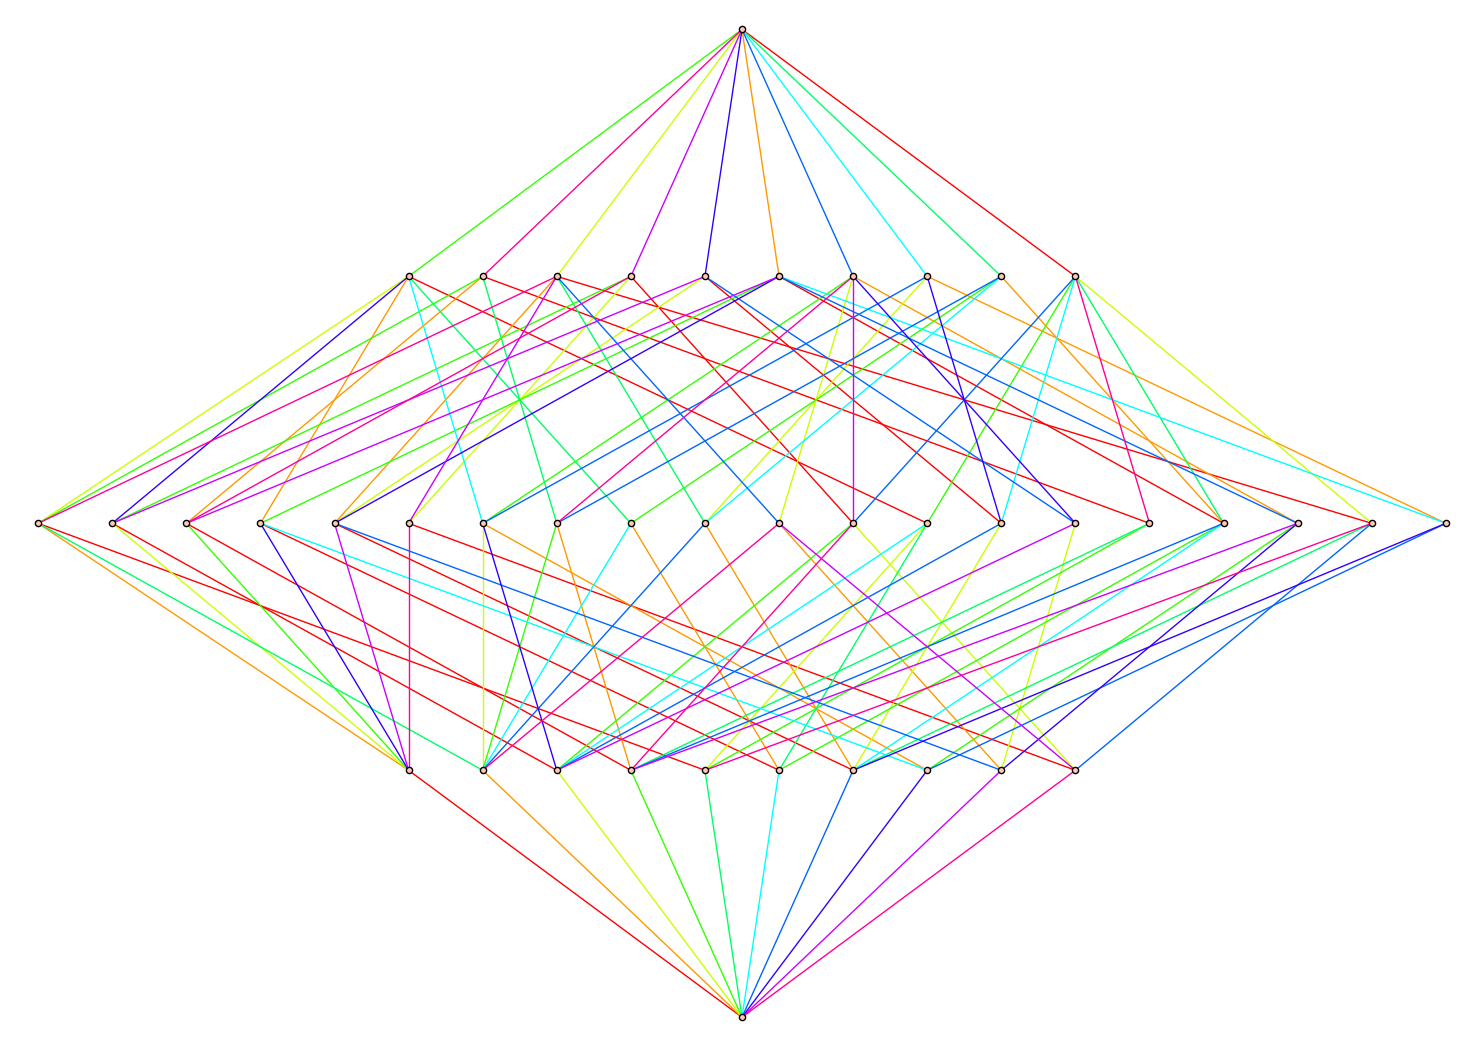
\includegraphics[width=7cm]{A4_interval.png}
	\caption{The interval $[1, (1,2)(2,3)(3,4)(4,5)]^{A_4}$ considering $A_4$ generated by all reflections, which label the edges by colour. Generated using \texttt{Sage} and \texttt{GAP} \cite{sagemath_2020, gap_2022}}
	\label{fig:A4_interval}
\end{figure}

These Coxeter elements are what we will use as the upper bound of our interval. In this case we consider $[1,w]^W$ with the set of all reflections $R$ as the generating set for $W$. See \cref{fig:A4_interval} for an example of such a poset. In principle there are many choices of Coxeter element depending on what order we multiply the elements of $S$. 
% However, we will see that in many cases these choices necessarily result in isomorphic $[1,w]^W$. We see that $S \subseteq R$, in particular $R$ generates $W$, since in the standard presentation of Coxeter groups all of $S$ are reflections.

\begin{definition}[Dual Artin group]
    For a given Coxeter group $W$ with Coxeter element $w in W$. Define $[1,w]^W$ as above, considering the set of all reflections $R$ as the generating set. The \emph{dual Artin group} $W_w$ is the poset group $G([1,w]^W)$ with $G$ defined as in \cref{def:poset_group}.
\end{definition}

It is known for finite \cite{bessis_dual_2003} and affine \cite{mccammond_sulway_artin_2017} cases that the dual Artin group is isomorphic to the Artin group $G_W$ (and thus that it does not depend on the choice of $w$). In general this is not known whether $G_W \cong G_w$ or whether the isomorphism class of $G_w$ depends on $w$.

\end{document}